\scanpage{170}
Fonc\uline{teurs fibres motiviques, et gps fondame}% word cut off by torn right edge; no further letters survive
\uline{motiviques}.

À examiner :

0)\quad VA
\figure{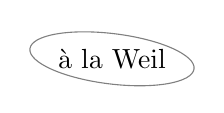
\begin{tikzpicture}[baseline=(w.base)]\node (w) at (0,0) {à la Weil};\draw[gray] (0,0) ellipse [x radius=1.05,y radius=.32,rotate=-7];\end{tikzpicture}}
\unsure{associées} aux motifs purs de poids impairs sur
\inserted{Conditions \unsure{de|\uline{de}|\deleted{de}} Hodge-Riemann\ldots}

\margin{OK\quad *}
\figure{
\begin{tikzpicture}\node[draw,circle,inner sep=3pt] {1};\end{tikzpicture}}
Extension \unsure{du|de} \unsure{groupe|groupes} \unsure{définie|définies|défini} par des \unsure{pts motiviques|places arithmétiques|places antiques}

Grou\uline{pe fondamental motivique}.

\figure{
\begin{tikzpicture}\node[draw,circle,inner sep=3pt] {2};\end{tikzpicture}}
Relations avec le corps de classes

\margin{OK}
\figure{
\begin{tikzpicture}\node[draw,circle,inner sep=3pt] {3};\end{tikzpicture}}
Cas du spectre d'un corps fini. Pts motiviques

parties à val. dans $\mathbb{R}$ ???

\margin{*}
4)\quad Rôle \unsure{du|des} \unsure{gpe|groupe|gps} \unsure{fondamental|fondamentaux} motivique pour la comparaison des réseaux canoniques
\diagram{$\left[\begin{array}{ll}
\text{dans Ch. de Hodge} & \left|\begin{array}{l}
\text{2 réseaux transcendant \unsure{pr.|prov.} \unsure{des|deux} places diff.}\\
\text{réseau transcendant et \unsure{réseau|réseaux} de Hodge}
\end{array}\right.\\[1em]
\text{dans Coh. $l$-adique} & \left|\text{2 réseaux transcendants}\right.
\end{array}\right]$}

5)\quad Relations \inserted{de 4} avec mes \unsure{notes|autres} \unsure{anciennes|anciens}

6)\quad \unsure{Fonction|Fonctions} $L$: équation fonctionnelle

\margin{OK}
7)\quad Structures \unsure{pratiques|positives|p-adiques}\ldots

\deleted{7}8)\quad Topologie à mettre sur $\mathbb{Z}$ \texttt{-{}-{}-{}-}

9)\quad Hyp. de Riemann \unsure{??}

\margin{Positivité à la Hodge en se ramenant à des questions de \uline{diviseurs} par éclatements, ou Variétés de drapeaux ??}
% archive sheet number: 169
